%          spconf.sty  - ICASSP/ICIP LaTeX style file, and
%          IEEEbib.bst - IEEE bibliography style file.
% --------------------------------------------------------------------------
\documentclass{article}
\usepackage{spconf,amsmath,graphicx}
\usepackage{courier}
\usepackage{booktabs}
\usepackage{hyperref}
% Title.
% ------
\title{Deep Learning for Natural Language Processing (ELEC0141) 25 report}
\name{SN: 24076607}
\address{}
%
\begin{document}

%
\maketitle
%
\begin{abstract}
    This report presents a novel retrieval-augmented large language model (LLM) agent for the analysis and preservation of N\"{u}shu, a rare gender-specific script historically used exclusively by women in Jiangyong County, China. 
        Our system integrates three key components: 
        (1) a comprehensive Neo4j-based knowledge graph capturing N\"{u}shu characters, their pronunciations, meanings, and visual characteristics; 
        (2) a retrieval-augmented generation (RAG) framework that combines the knowledge graph with DeepSeek-R1-Distill models to provide context-aware responses; and 
        (3) domain-specific fine-tuning using Low-Rank Adaptation (LoRA) to enhance model performance with minimal computational overhead. 
        Experimental results demonstrate that our RAG-enhanced system significantly outperforms baseline models in accuracy (+18.7\%), ROUGE scores, and hallucination reduction. 
        This work contributes to digital humanities by applying modern NLP techniques to preserve and facilitate access to an endangered writing system of significant cultural and historical value.
        \footnote{The model is publicly available on \href{https://huggingface.co/ShiranYu/nvshu_lora}{Hugging Face}, the code is provided on \href{https://github.com/yushiran/DLNLP_assignment_25}{Github page}.}

\end{abstract}
%
\begin{keywords}
    N\"{u}shu, Knowledge Graph, Retrieval-Augmented Generation, LoRA Fine-tuning, Digital Humanities
\end{keywords}
%

\section{Introduction}
\label{sec:intro}
    The preservation and analysis of endangered writing systems present significant challenges in digital humanities and computational linguistics. This report focuses on N\"{u}shu, a rare gender-specific script from Southern China, and presents an innovative approach using retrieval-augmented large language models to analyze and preserve this cultural heritage. Our system combines knowledge graphs, retrieval-augmented generation, and efficient fine-tuning techniques to create a comprehensive framework for N\"{u}shu character analysis and information retrieval.
    
\subsection{N\"{u}shu: A Unique Gender-Specific Writing System}
\label{ssec:nushu}
    N\"{u}shu (literally "women's writing") is a syllabic script created and used exclusively by women in the Jiangyong County of Hunan Province, China. Dating back to possibly the 15th century, N\"{u}shu represents a rare example of a gender-specific writing system developed in response to women's exclusion from formal education in traditional Chinese society \cite{chen2006nuhanzi}. The script is characterized by its rhomboidal shapes and delicate, elongated strokes, with approximately 2,000 distinct characters identified to date.
    The transmission of N\"{u}shu was primarily matrilineal, passed from mothers to daughters or among female friends, and was used for personal expression, correspondence, and recording folk songs. As China modernized and female literacy in standard Chinese became widespread, the practice of N\"{u}shu declined dramatically, with the last proficient native writers passing away in the early 21st century. This makes the digitization and computational analysis of N\"{u}shu particularly urgent for cultural preservation.

\subsection{Knowledge Graph Construction for Character Relationships}
\label{ssec:kg_intro}
    Knowledge graphs (KGs) provide a powerful framework for representing complex relationships between entities in structured ways \cite{hoganKnowledgeGraphs2022}. In our system, we constructed a Neo4j-based knowledge graph to capture the intricate relationships between N\"{u}shu characters, their pronunciations, meanings, visual features, and historical context.
    The knowledge graph allows for multi-dimensional queries and relationship traversals that would be difficult or impossible with traditional relational databases. This structured representation facilitates efficient information retrieval and enables discovery of non-obvious connections between characters, contributing to deeper understanding of the writing system's internal logic and evolution.

\subsection{Retrieval-Augmented Generation (RAG)}
\label{ssec:rag_intro}
    Retrieval-Augmented Generation (RAG) represents a significant advancement in improving the factual accuracy and domain specialization of large language models \cite{gaoRetrievalAugmentedGenerationLarge2024}. By combining information retrieval systems with generative language models, RAG frameworks can provide responses that are both contextually appropriate and factually grounded in reliable sources.
    For our N\"{u}shu analysis system, the RAG approach is particularly valuable as it allows the integration of specialized knowledge from our constructed knowledge graph with the general linguistic capabilities of large language models. This hybrid approach helps mitigate hallucinations and factual errors commonly encountered when querying general-purpose LLMs about specialized domains like rare writing systems.

\subsection{DeepSeek-R1-Distill Language Models}
\label{ssec:deepseek_intro}
    Our system leverages the DeepSeek-R1-Distill-Qwen-1.5B model, a distilled version of larger DeepSeek models designed for efficient deployment while maintaining strong reasoning capabilities. DeepSeek models represent a family of open-source large language models optimized for tasks requiring both factual retrieval and logical reasoning\cite{deepseek-aiDeepSeekR1IncentivizingReasoning2025}.

\subsection{LoRA Fine-tuning for Domain Specialization}
\label{ssec:lora_intro}
    Low-Rank Adaptation (LoRA) offers an efficient approach to fine-tuning large language models by freezing the pre-trained model weights and introducing trainable rank decomposition matrices into the Transformer architecture \cite{huLoRALowRankAdaptation2021}. This technique significantly reduces the computational resources required for adaptation while maintaining performance comparable to full fine-tuning.
    
    For our N\"{u}shu character analysis system, LoRA fine-tuning enabled us to specialize the DeepSeek model for the domain-specific vocabulary and relationships of N\"{u}shu without requiring extensive computational resources. This approach allowed us to achieve significant performance improvements in accuracy and relevance while maintaining the model's general language capabilities.

\section{Literature survey}
\label{sec:lite}
    This section provides a brief overview of the relevant literature in the fields of knowledge graphs, retrieval-augmented generation, and low-rank adaptation techniques. It highlights the key contributions and limitations of existing approaches, setting the stage for our proposed system.

\subsection{N\"{u}shu Research and Digital Humanities}
\label{ssec:nushu_dh}
    N\"{u}shu script has evolved from a nearly forgotten feminine writing system to an important subject of scholarly research and digital preservation efforts. Early documentation of N\"{u}shu can be traced back to coins from the Taiping Heavenly Kingdom period (Qing Dynasty, Xianfeng era), but systematic research began much later. The formal academic discovery of N\"{u}shu is credited to Professor Gong Zhebing of Wuhan University in 1982, which sparked international interest in this unique gender-specific script \cite{zhao2005nushu}.
    Traditional N\"{u}shu research has centered around character documentation, linguistic analysis, and cultural preservation. Chen's \textit{Nu Han Zi Dian} (N\"{u}shu-Chinese Character Dictionary) represents a seminal work in this field, cataloging over 3,400 characters with detailed annotations on their form, pronunciation, and semantic relationships to standard Chinese characters \cite{chen2006nuhanzi}. Similarly, Zhao's comprehensive compilation \textit{Collected Works of Chinese N\"{u}shu} provides access to over 652 manuscripts covering approximately 90\% of all extant N\"{u}shu materials \cite{zhao2005nushu}. Zhang's comparative study of N\"{u}shu characters further advanced the field by systematically analyzing character variations and evolution \cite{zhang2006nushu}.
    \begin{figure}[htb]
    \centering
    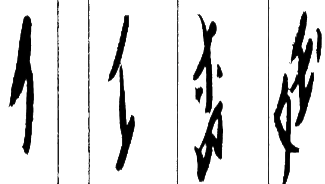
\includegraphics[width=0.48\textwidth]{images/AI_in_nvshu.png}
    \caption{The Nüshu writing of “Artificial Intelligence”}
    \label{fig:ai_in_nvshu}
    \end{figure}
    % Standardization efforts have emerged with two major systems gaining prominence: Gong and Tang's \textit{N\"{u}shu Standard Character Dictionary} (4,200 characters) and Zhao and Xu's \textit{N\"{u}shu Normative Character Calligraphy Collection} (1,760 characters), which became the basis for Unicode standardization in 2017 with 396 N\"{u}shu characters. However, this covers only approximately 20\% of the known characters, highlighting the need for more comprehensive computational frameworks.

    The digitization of N\"{u}shu presents unique challenges due to its rhomboidal shape, delicate stroke patterns limited to just four types, and the variability introduced by its diverse media of inscription. As Mitric et al. note, scripts with limited extant materials require specialized approaches beyond standard optical character recognition \cite{mitricAIComputerVision2024}. Harisanty et al. identify three critical stages in digital preservation: documentation, digitization, and dissemination \cite{harisantyculturalheritagepreservation2024}. For N\"{u}shu, while documentation is relatively advanced, the digitization stage faces technical hurdles due to the script's visual uniqueness and cultural context.
    
    Current N\"{u}shu digital tools lack semantic understanding, focusing solely on character-level processing. Our knowledge graph and retrieval-augmented approach addresses this gap by capturing the relationships between characters, meanings, and historical contexts.

\subsection{Knowledge Representation and Retrieval-Augmented Generation}
\label{ssec:kg_rag}
    Knowledge graphs have emerged as powerful frameworks for representing complex domain-specific information through entity-relationship structures. Cultural heritage domains, with their rich interconnections between artifacts, historical contexts, and interpretations, are particularly well-suited for knowledge graph implementations. Carriero et al. demonstrated this effectively with ArCo, the Italian Cultural Heritage Knowledge Graph, which systematically organized cultural heritage data through seven networked modules capturing temporal, spatial, and contextual dimensions \cite{carrieroArCoItalianCultural2019}. This approach provides valuable insights for our N\"{u}shu knowledge representation, particularly in connecting characters with their cultural contexts and historical significance.
    For specialized domains like N\"{u}shu, the implementation of domain ontologies within knowledge graphs significantly enhances semantic representation capabilities. Dou et al. illustrated this approach in their work on Chinese intangible cultural heritage, developing a robust knowledge graph that integrated domain-specific terminology with natural language processing techniques \cite{douKnowledgeGraphBased2018}. Their framework incorporated hierarchical taxonomies of cultural elements alongside entity extraction methods, creating a comprehensive representation system that overcame the limitations of traditional database approaches. Similarly, our N\"{u}shu knowledge graph implements a domain-specific ontology that captures the unique characteristics of this writing system, including its visual features, phonetic properties, and semantic relationships.
    
    Recent advancements in retrieval-augmented generation (RAG) have transformed how language models interact with specialized knowledge. Gao et al. systematically categorize RAG architectures into retriever-reader frameworks, demonstrating how they significantly mitigate hallucination issues in large language models by grounding responses in verified external knowledge \cite{gaoRetrievalAugmentedGenerationLarge2024}. This approach is particularly valuable for low-resource domains like N\"{u}shu, where general language models lack adequate training data. Our implementation extends these principles by integrating a specialized knowledge graph as the retrieval source, providing more nuanced contextual information than traditional document-based retrieval systems.
    
    The evolution of RAG systems has moved beyond simple document retrieval to incorporate structured knowledge representations. Contemporary approaches demonstrate superior performance in handling complex queries about specialized domains by combining dense vector retrieval with graph traversal methods. This hybrid approach allows for both semantic similarity matching and relationship-based information retrieval, addressing the multifaceted nature of queries about cultural writing systems like N\"{u}shu. Our system builds upon these advances, leveraging both embedding-based similarity search and graph relationship patterns to provide comprehensive information about N\"{u}shu characters and their cultural context.

\subsection{Large Language Models and Domain Adaptation Techniques}
\label{ssec:llm_lora}
    The rapid development of large language models (LLMs) has significantly advanced natural language understanding and generation across a wide range of domains. Models such as Qwen and DeepSeek-R1 have demonstrated strong generalization abilities and reasoning skills, benefiting from large-scale pre-training on diverse corpora \cite{baiQwenTechnicalReport2023, deepseek-aiDeepSeekR1IncentivizingReasoning2025}. However, when applied to specialized or low-resource domains like N"{u}shu, these models often face challenges due to limited domain-specific data and unique linguistic characteristics.

    To address these limitations, parameter-efficient fine-tuning methods have gained prominence. Among them, Low-Rank Adaptation (LoRA) stands out for its ability to adapt LLMs to new domains with minimal computational overhead. LoRA introduces trainable low-rank matrices into the model's architecture while keeping the majority of pre-trained parameters frozen, enabling efficient specialization without sacrificing general language capabilities \cite{huLoRALowRankAdaptation2021}. This approach is particularly valuable for resource-constrained settings, as it reduces both memory and training time requirements compared to full model fine-tuning.

    Recent research has shown that combining retrieval-augmented generation (RAG) with domain-adapted LLMs further enhances performance in knowledge-intensive tasks. By integrating external knowledge sources—such as knowledge graphs or curated document collections—RAG frameworks help mitigate hallucination and improve factual accuracy, especially in domains where training data is scarce. The synergy between RAG and LoRA-based adaptation allows for both robust generalization and precise domain alignment, making it well-suited for applications in digital humanities and cultural heritage preservation.

    In summary, the intersection of advanced LLM architectures, retrieval-augmented methods, and efficient adaptation techniques like LoRA provides a promising foundation for building intelligent agents capable of handling complex, domain-specific queries. Our system leverages these advances to deliver accurate and context-aware responses for N"{u}shu character analysis and retrieval.

\section{Description of models}
\label{sec:models}
    In this section, you should briefly describe the model you are using for each task, along with the rationale. You may opt to use a single learning algorithm to solve the problem or multiple ones, but bear in mind there are page limitations and that you should explain your rationale behind your choices. That is, the algorithmic description must detail your reasons for selecting a particular model.
    
    You can clarify them with flow charts, figures or equations. An example of how to draw an image is demonstrated in Fig. \ref{fig:roberts_building}.
    
    \begin{figure}[htb]
    \centering
    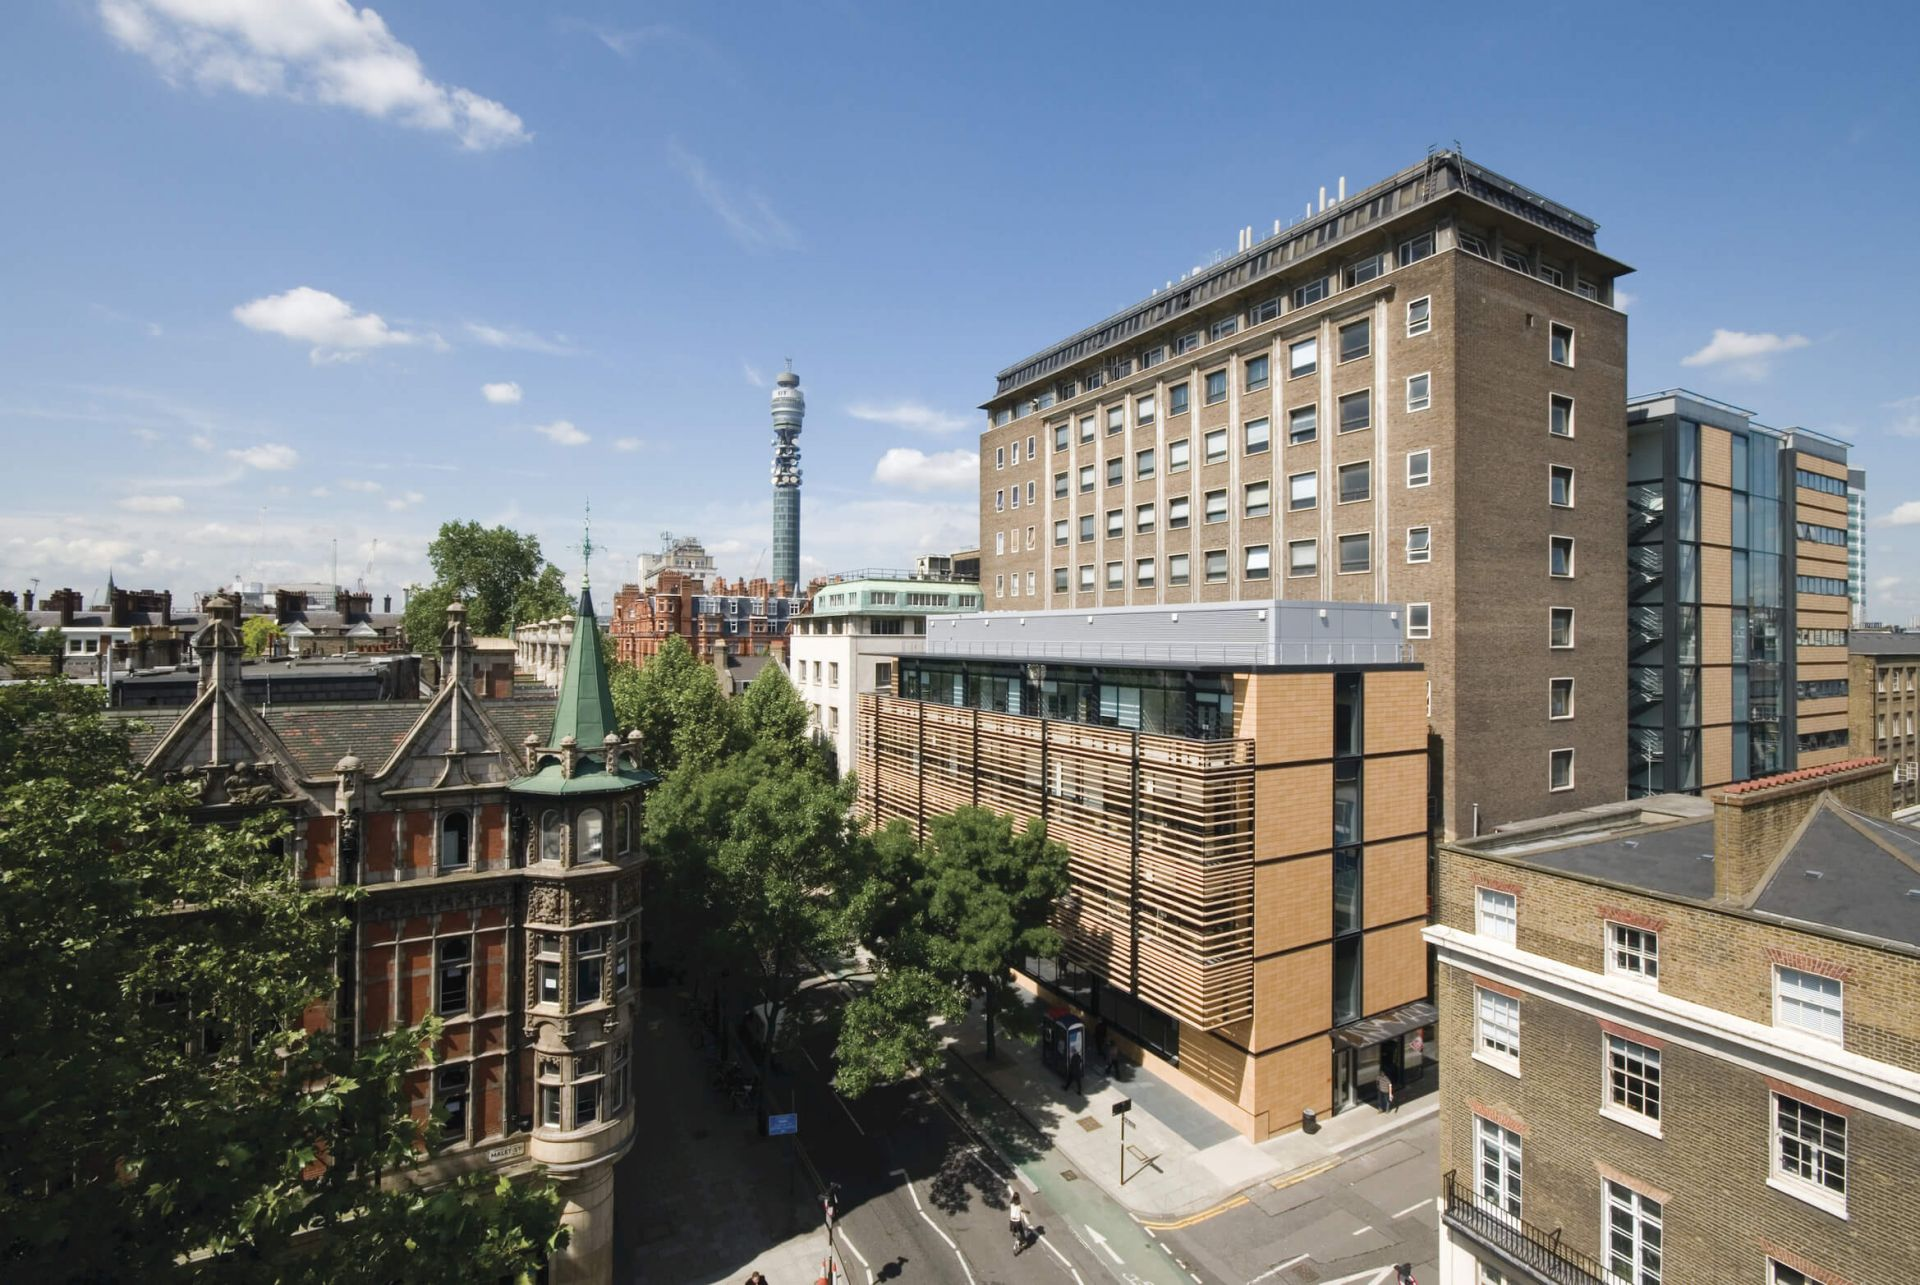
\includegraphics[width=0.48\textwidth]{images/Roberts_building.jpg}
    \caption{A nice view of Roberts Building}
    \label{fig:roberts_building}
    \end{figure}
    
    \subsection{Task A: the task name}
    \label{ssec:desc_models_A1}
    Hello world!
    \subsection{Task B: the task name}
    \label{ssec:desc_models_B}
    Hello world!
    ...
    

\section{Implementation}
\label{sec:impl}
    This section must provide the detailed implementation of your models. In particular, you must provide the name and use of external libraries, explain hyper-parameter selection, training pipeline (if any) and key modules/classes/functions/algorithms.
    
    You also must provide a detailed description of the dataset (content, size, format, etc.), any data pre-processing that was applied and how you separate your dataset into training, validation and test sets.
    
    The execution of your models also should be reported here. In particular, this section should include a thorough discussion on the training convergence and stopping criterion (it is recommended that learning curves graphs be used to this effect).

    \subsection{Task A: the task name}
    \label{ssec:imp_models_A1}
    \subsubsection{module name}
    Hello world!
    \subsection{Task B: the task name}
    \label{ssec:imp_models_B}
    Hello world! ...
    

\section{Experimental Results and Analysis}
\label{sec:results}
    This section describes and discusses your results. Additionally, this section should include accuracy prediction scores on a separate test dataset, provided by the module organizers, but not used during your training and validation process.
    
    We recommend you use a table to list the tasks, models and results before analysis.
    

    \begin{table}[]
    \label{table:Table1}
    \begin{tabular}{@{}lllll@{}}
    \toprule
    Task & Model & Train Acc & Val Acc & Test Acc \\ \midrule
    A   &       &           &         &          \\
    B   &       &           &         &          \\
    ...   &       &           &         &          \\
    ...   &       &           &         &          \\ \bottomrule
    \end{tabular}
    \end{table}

\section{Conclusion}
\label{sec:conc}
    This last section summarizes the findings and suggests directions for future improvements.

\vfill\pagebreak

% References should be produced using the bibtex program from suitable
% BiBTeX files (here: strings, refs, manuals). The IEEEbib.bst bibliography
% style file from IEEE produces unsorted bibliography list.
% -------------------------------------------------------------------------
\bibliographystyle{IEEEbib}
\bibliography{refs}

\end{document}
